% Dữ liệu minh họa, không chứa thông tin cá nhân.
\begin{ex}
Tính đạo hàm của hàm số $f(x)=x^2$.
\choice{$x$}{\True $2x$}{$x^3$}{$2$}
\loigiai{Ta có $f'(x)=2x$.}
\end{ex}

\begin{ex}
Xét các khẳng định sau về hàm số $y=x^2$.
\choiceTF{\True Đồ thị đi qua gốc tọa độ.}{Hàm số nghịch biến trên toàn trục số.}{\True Hàm số chẵn.}{Đồ thị là đường thẳng.}
\loigiai{Đúng, sai, đúng, sai.}
\end{ex}

\begin{ex}
Tính $\int_0^1 2x\,dx$.
\shortans{1}
\loigiai{$\int_0^1 2x\,dx=[x^2]_0^1=1$.}
\end{ex}

\begin{ex}
Quan sát hình vẽ và xác định bán kính đường tròn.
\begin{center}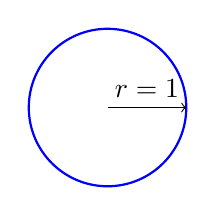
\begin{tikzpicture}\draw[blue,thick] (0,0) circle (1);\draw[->] (0,0)--(1,0) node[midway,above]{$r=1$};\end{tikzpicture}\end{center}

\includegraphics[width=4cm]{diagram.png}
\loigiai{Bán kính bằng $1$.}
\end{ex}
